\chapter{"Квазипланковский" спектр капиллярной турбулентности на поверхности жидкого водорода}


В турбулентном каскаде область накачки и диссипации значительно разнесены в пространстве волновых векторов. Наличие диссипативной области является необходимым условием для установления турбулентного каскада. В диссипативной области турбулентного распределения механическая энергия волн переходит в тепло в результате вязких потерь. Энергия в диссипативную область поступает в результате нелинейного взаимодействия волн с гармониками из инерциального интервала. Распределение энергии в диссипативной области определяется характером волнового взаимодействия как внутри области, так и с волнами более низкой частоты \cite{Ryzhenkova1990}. 
В этой главе представлены результаты исследования распределения энергии по частоте в диссипативной области турбулентного каскада в системе капиллярных волн на поверхности жидкого водорода. При изучении волновой турбулентности жидкий водород выгодно отличается от воды в пять раз более низким коэффициентом кинематической вязкости и в три раза большим коэффициентом нелинейности капиллярных волн, который оценивается как $V \sim (\sigma / \rho^3)^{1/4}$ . Таким образом, при равных угловых амплитудах волн на частоте накачки относительная ширина инерционного интервала, оцениваемая из равенства времен вязкого затухания волн, оказывается в три раза больше для водорода. 

\section{Экспериментальная методика} %\label{sect1_1}
Экспериментальная установка состоит из гелиевого криостата (рис. \ref{img:cryostat}), в вакуумной полости которого расположена оптическая ячейка (рис. \ref{img:opt_cell} ), системы возбуждения колебаний на поверхности жидкости и оптической системы их регистрации. Медный цилиндрический стакан глубиной 6 мм и внутренним диаметром 60 мм был установлен внутри ячейки. На расстоянии 4 мм над стаканом располагается металлическая пластина. Газообразный водород сконденсируется в стакан до максимального уровня. Радиоактивная мишень (молибденовая пластина, покрытая слоем тритида титана), расположенная на дне стакана, ионизирует жидкий водород. В присутствии постоянного электрического напряжения около 1 кВ между стаканом и верхней пластиной, положительно заряженные ионы собираются под поверхностью жидкого водорода, образуя квазидвумерный слой. Волны на поверхности жидкого водорода возбуждаются дополнительным к постоянному переменным напряжением с максимальной амплитудой около 100 В, приложенным к стакану  \cite{Brazhnikov_IET}.
 
\begin{figure}[ht] 
 \center
 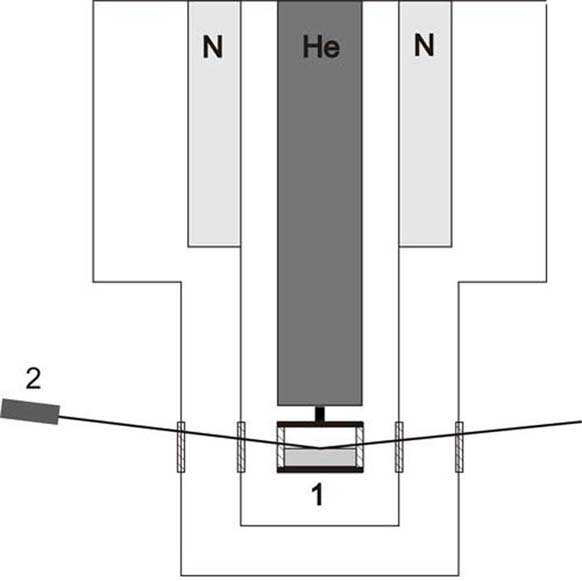
\includegraphics [scale=0.4] {article1/kriostat.jpg}
 \caption{Схематичная конструкция криостата.
 1 – экспериментальная ячейка, 2 – лазер.} 
\label{img:cryostat} 
 
\end{figure}


\begin{figure}[ht] 
 \center
 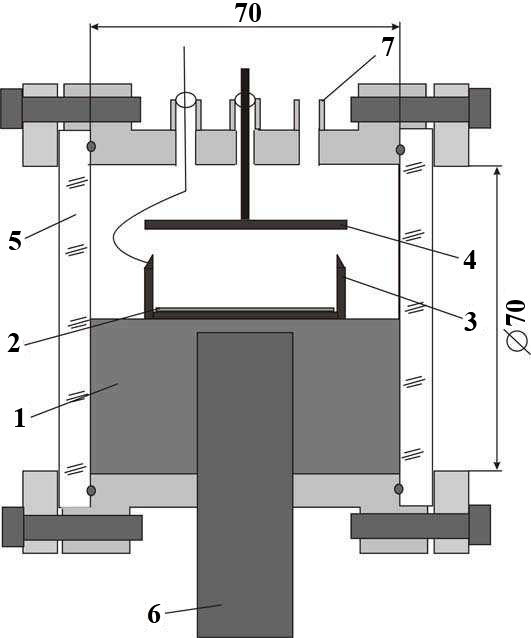
\includegraphics [scale=0.4] {article1/cell.jpg}
 \caption{Схематичная конструкция экспериментальной ячейки. 
 1 – текстолитовый брусок, 2 – радиоактивная мишень, 3 – медный контейнер, 4 – верхняя обкладка конденсатора, 5 – кварцевое окно, 6 - медный хладопровод, 7 – капилляр для набора водорода.} 
\label{img:opt_cell} 
\end{figure}

Использование переменного электрического поля позволяет возбуждать на поверхности капиллярные волны хорошо контролируемой силой. В этих экспериментах в качестве переменного возбуждающего напряжения были использованы низкочастотные случайные сигналы, сосредоточенные в полосе частот. Эти сигналы были синтезированы обратным Фурье-преобразованием случайного набора фаз и прямоугольного амплитудного спектра, который везде равен нулю кроме заданного частотного интервала накачки (см. рис. \ref{img:spectra_pump}). Фрагмент сигнала накачки приведен на рис. \ref{img:frag_pump}
	
\begin{figure}[ht] 
 \center
 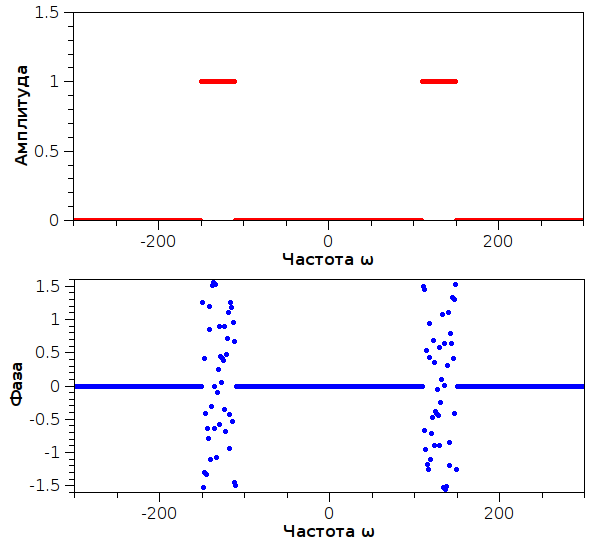
\includegraphics [scale=0.75] {article1/ftt-gen1.png}
 \caption{Частотное распределение амплитуды (верхний график) и пример частотного распределения фазы (нижний рисунок) сигнала, использующегося в качестве накачки.} 
\label{img:spectra_pump} 
\end{figure}

\begin{figure}[ht] 
 \center
 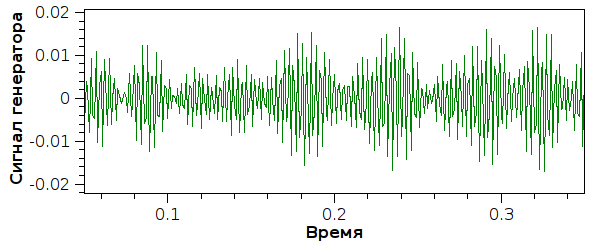
\includegraphics [scale=0.75] {article1/fft-gen2.png}
 \caption{Фрагмент сигнала накачки.} 
\label{img:frag_pump} 

\end{figure}

Для регистрации волн на поверхности жидкости использовался метод отражения лазерного луча. Лазерный луч падает под малым скользящим лучом (около 0.2 рад) на поверхность жидкости. Отраженный луч фокусируется линзой на фотодетектор. Напряжение на фотодетекторе усиливается и оцифровывается 24 битным аналого-цифровым преобразователем (ЦАП) с частотой дискретизации около 100 кГц. Волны регистрируются в режиме "широкого луча"{}, когда размер лазерного луча больше, чем характерная длина волны. Энергия отраженного лазерного луча $P(t)$ в этом режиме пропорциональна квадрату отклонения поверхности $\eta(t)$ \cite{Brazhnikov_bound_freq}. По этой причине в дальнейшем не делается разницы между спектром корреляционной функции отклонения поверхности $<|\eta_\omega^2|>$ и энергией отраженного лазерного луча $<P_\omega^2>$. Более подробно эта методика измерения описана в \cite{Brazhnikov_IET}.

	Максимальная угловая амплитуда волны, которая может быть зарегистрирована в эксперименте, ограничена размером оптических окон криостата и приблизительно равна 0.05 рад.

\section{Экспериментальные результаты и обсуждение} %\label{sect1_1}
 Капиллярные волны возбуждались случайной силой в частотном диапазоне 39-103 Гц. Средний квадрат возбуждающего напряжения менялся от $V_p = 0$ В, т.е. отсутствие накачки, до $V_p = 30$ В, Ограничение связано с максимальной угловой амплитудой волны. На рис. \ref{img:hydr_specrta_dlog} показан пример Фурье-спектра для отраженной энергии лазерного луча $P_\omega^2$ при разных амплитудах возбуждающей силы. На рис \ref{img:hydr_specrta_dlog} хорошо видна область накачки в низкочастотной части спектра. За областью накачки следует инерционный интервал - относительно широкая частотная область, где видна степенная зависимость спектра $P_\omega^2$. Ширина инерционного интервала зависит от амплитуды накачки. Когда поверхность возбуждается слабо (переменное напряжение $V_p = 4$ В) область диссипация начинается рядом с областью накачки и инерционный интервал не наблюдается. Увеличение силы накачки приводит к уширению инерционного интервала, высокочастотная граница инерционного интервала $\omega_b$ смещается к высоким частотам. Наиболее широкий инерционный интервал с границами от $\approx 0.3$ кГц, до $\omega_b \approx 4$ кГц наблюдается при максимальном напряжении накачки $V_p = 30$ В. На частотах выше высокочастотной границы инерционного интервала колебания поверхности затухают из-за вязких потерь, кривая $P_\omega^2$ идет вниз гладко и уходит ниже уровень аппаратных шумов.
 
 \begin{figure}[ht] 
 \center
 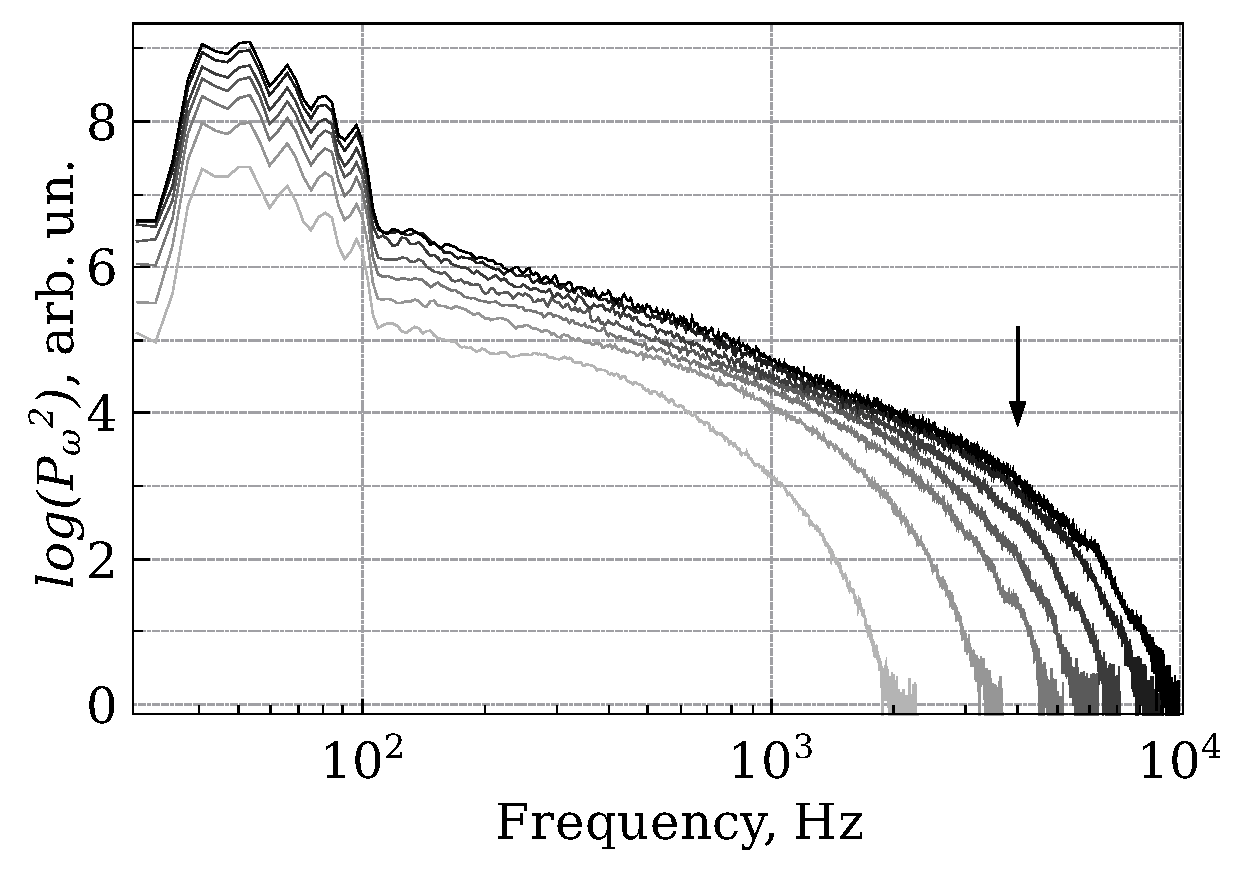
\includegraphics [scale=.8] {article1/spectra_dlog.eps}
 \caption{Спектры поверхностных колебаний $P^2_\omega$, возбужденных случайной силой в частотном диапазоне 39-103 Гц при разных амплитудах возбуждающей силы. Среднеквадратичное значение возбуждающего напряжения $V_P$ меняется от 4 до 30 В. Более темные линии соответствуют большей силе накачки. Стрелкой показана высокочастотная граница инерционного интервала $\omega_b \approx 4$ кГц при накачке 30 В.} 
 \label{img:hydr_specrta_dlog} 
\end{figure}

Турбулентные спектры, перестроенные в полулогарифмическом масштабе на рис. \ref{img:hydr_specrta_log}, показывают, что убывание амплитуд волн с частотой выше высокочастотной границы инерционного интервала может быть достаточно хорошо описано экспоненциальной функцией $P_\omega^2 \sim	\omega^-s e^{-\omega/\omega_d}$ в некотором интервале частот. Полученный параметр $\omega_d$ оказывается значительно меньше, чем частоты из интервала подгонки, что разумно для планковского распределения. Например спектр, полученный при амплитуде переменного напряжении накачки $V_p = 26$ В хорошо приближается экспоненциальной функцией в диапазоне 5-9 кГц с $\omega_d \approx 0.6$ кГц. К сожалению, узкий интервал подгонки не позволяет установить показатель степени s "квазипланковского" распределения достаточно точно. Полученные значения $\omega_d$ в несколько раз меньше, чем видимая граница между инерционным интервалом и диссипативной области(см. рис. \ref{img:hydr_specrta_dlog}). Это несоответствие можно отнести к определенной степени свободы в определении граничной частоты, которая может быть перенормирована с помощью некоторой константы.

\begin{figure}[ht] 
 \center
 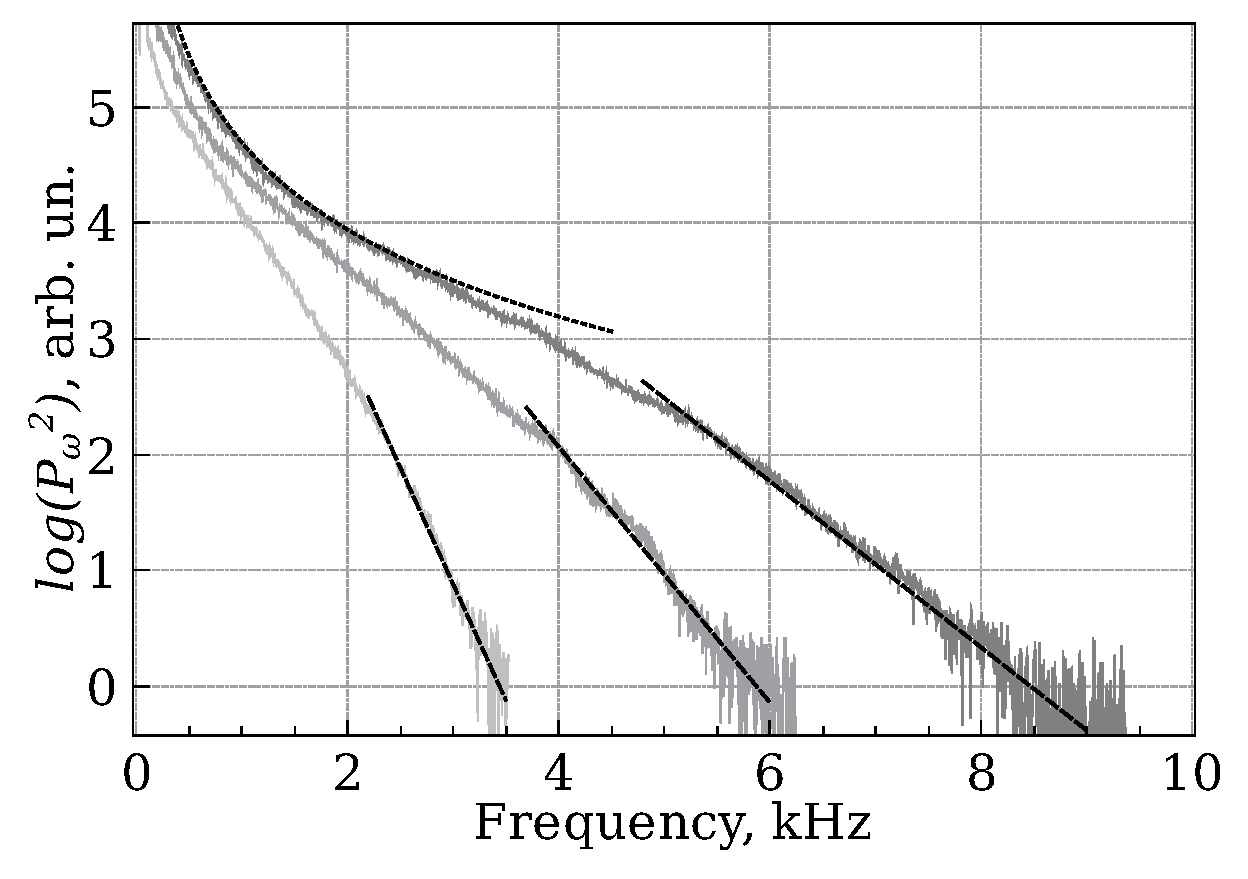
\includegraphics [scale=0.8] {article1/spectra_log.eps}
 \caption{Спектры $P^2_\omega$ для уровней накачки $V_p = 8$ В (светло серая линия), $16$ В (серая линия) и $26$ В (темно-серая линия) в полулогарифмическом масштабе. Линией из точек показан степенной закон $\sim \omega^{-2.8}$, пунктирной линией - подгонка функцией $ \sim e^{-\omega/\omega_d}$. $\omega_d$ примерно равен 0.2, 0.4 и 0.6 для $V_p$ = 8, 16 и 26 В соответственно.} 
 \label{img:hydr_specrta_log} 
\end{figure}

	Характерная частота $\omega_d$, оцененная с помощью подгонки экспоненциального затухания в диссипативной области к экспериментальным данным, растет с увеличением амплитуды возбуждающей силы. Для измерения уровня возбуждения использовался отклик поверхности $\eta_0$, а именно абсолютное значение $P_\omega$ на частоте 53 Гц (положение максимума распределения $P_\omega^2$ внутри области накачки). Величина $\eta_0$ прямо пропорциональна средней высоте волны на той же самой частоте. На рис. \ref{img:hydr_wd} показано, что зависимость граничной частоты от величины возбуждения может быть описана степенным законом $\omega_d(\eta_0) \sim	\eta_0^m$ со значение показателя $m = 0.85 \pm 0.05$. Необходимо заметить, что подгонка экспоненциальных спектров с помощью "квази-Планка" с малым ненулевым $s$ ($|s| \le 2$) слабо влияет на полученный параметр $\omega_d$ (изменение менее 20\%). Эта поправка не изменит показатель степени $m$ в пределах погрешности.

	Наблюдаемый показатель $m \approx 0.85$ значительно отличается от ожидаемого $m = 12/5$ (см. параграф \ref{subsect_hiFreqBound} введения). Стоит отметить, что в случае турбулентных каскадов, возбужденных монохроматической силой, измеренная в \cite{Brazhnikov2001} граничная частота находится в хорошем соответствии с ожиданиями $\omega_d(\eta) \sim \eta^{1.3}$.
	
\begin{figure}[ht] 
 \center
 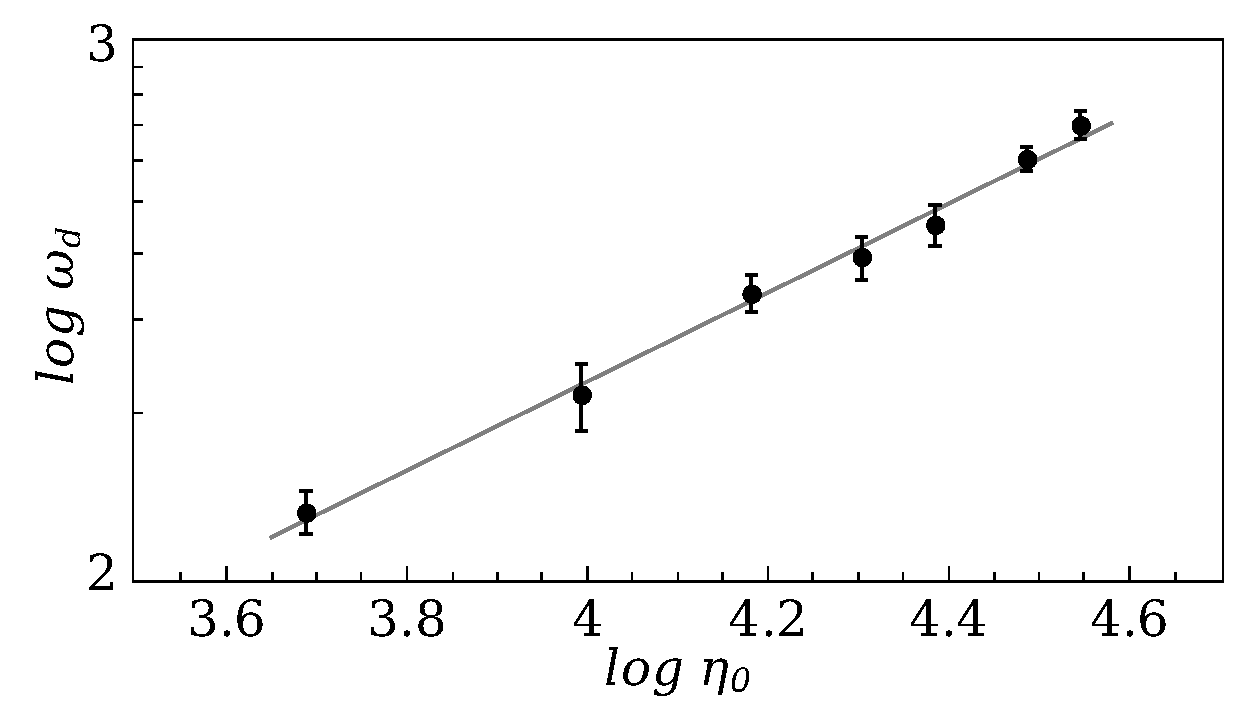
\includegraphics [scale=0.7] {article1/wd.eps}
 \caption{
 Зависимость частоты вязкого затухания диссипативной области $\omega_d$ (черные точки) от средней высоты низкочастотной волны $\eta_0$, сплошная линия - подгонка функцией $\eta_0^{0.85}$. }
 \label{img:hydr_wd} 
\end{figure}
\section{Выводы}% \label{sect2_4}

Впервые наблюден переход от степенного спектра Колмогова-Захарова в инерционном интервале к "квазипланковскому"{} распределению $\omega^{-s}e^{-\omega/\omega_d}$ в области диссипации энергии в турбулентном распределении системы капиллярных волн. Экспоненциальный спад в области диссипации $\omega/\omega_d \gg 1$ соответствует теоретическому ожиданию и качественно соответствует численным вычислениям \cite{Ryzhenkova1990}. Граница вязкого затухания $\omega_d$ растет с увеличением амплитуды накачки и зависит от средней высоты волны $\eta_0$ на частоте накачки как $\omega_d \sim \eta^{0.85 \pm 0.05}$. Однако наблюденная зависимость отличается от теоретически ожидаемой, показатель степени почти в три раза больше предсказанного значения.



\clearpage

